\documentclass{article}
\usepackage[utf8]{inputenc}
\usepackage{hyperref}
\setlength{\columnsep}{1cm}
\usepackage[margin=0.5in]{geometry}

\title{Deep Learning Course - Final Project}
\author{Nitsan BenHanoch (208585927), Nir Koren (316443902), Tsvi Tabach (311292304)}
\date{Submitted as a final project report for the DL course, BIU, 2024}

\usepackage{natbib}
\usepackage{graphicx}
\usepackage{float}
\usepackage[normalem]{ulem} % Import ulem and preserve \emph for italics

\begin{document}

\maketitle

\section{Introduction}

Deep-Learning in healthcare is a hot topic. As deep neural networks become increasingly involved in patient care, these networks must meet several requirements. Such requirements include high precision rate, transparency in their decision-making, and performing effectively even when valuable data is missing.

\subsection{The Dataset}
Kaggle's chest-xray-pneumonia dataset consists of 5,856 lungs X-Ray images of men and children. Each image is labeled either "healthy", "bacterial-infected" or "viral-infected". The data is split between train/set sets. One important issue to note is the classes are not balanced; each set contains a different ratio of images from the different classes.

\subsection{Our Tasks}
In this project, we demonstrate several different deep-learning techniques we learned during the course.

\textbf{Task 1.a. Binary Classification}: we train a CNN on healthy/sick labeled x-ray images of human lungs;

\textbf{Task 1.b. Multiclass classification}: we further improve the CNN to distinguish between bacterial/viral infection;

\textbf{Task 2. Embedding Space:} we apply KNN and t-SNE on embedding vectors we get from the aforementioned networks;

\textbf{Task 3. Anomaly Detection:} having trained on healthy lungs alone, we use auto-encoders to tell if lungs are sick;

\textbf{Task 4. Explainability}: we decipher the model's decision making, e.g. what's important to each layer and neuron.


\subsection{Related Works}
Previous research, such as \href{https://arxiv.org/pdf/1711.05225.pdf}{CheXNet}, study by Rajpurkar et al. (2017), has shown the advantage of using CNN in medical diagnostics. The model proposed in the paper used CNN to output probability of pneumonia with a heat-map localizing the pneumonia areas from chest X-ray images.

\
\section{Task 1.a: Binary Classification}

\subsection{Solution}
\subsubsection{The Task}
In this task, we treat both bacterial and viral images as
\textit{sick}, and train a model to classify \textit{healthy}/\textit{sick} lungs x-ray.

\subsubsection{General approach}
We use several convolution layers, followed by a few dense layers. It is the field's classic and go-to way to classify images. Furthermore, the limited dataset size (approximately 5K images) posses a serious restriction on the complexity of the network, as overly powerful architectures risk significant over-fitting.

\subsubsection{Design}

Our network's architecture mimics the great: we took inspiration from the architecture of the VGG networks family. We tailored their layer sizes to our needs after thorough experimentation, maximizing accuracy, while battling over-fitting. The final network structure is portrayed in Figure~\ref{fig:model_1}.

\textbf{Platform:} we built the model as a Keras Sequential on a kaggle notebook. It ran for $\sim$30 minutes using a P100 GPU. 

\textbf{Loss:} we used binary-crossentropy, as it's classic in the context of binary classification, and it worked for us. 

\textbf{Optimizer:} we used Adam with initial learning rate of 1e-4, but also installed a callback to further lower it on plateau.

\textbf{The Splits}: The train and the 16-images given val were concatenated and re-split into 80\% train and 20\% validation.

\textbf{Limited dataset size:} as said, we only had a few thousand images to train on.
We applied many forms of augmentation (e.g. shear, shift, rotation, brightness, zoom) to compensate for the lack of data, making room for a deeper network while avoiding over-fitting. We also limited the number of epochs; we found that lowering the learning-rate too much, to squeeze more "improving" epochs, actually hurt the the network's accuracy measured on the test set.

\textbf{Class imbalance:} the sets had different distributions of labels.
We removed excess data from the train/val sets until each class appeared 50\%; we found that to be more effective than assigning weights. The test-set, having a 62.5\% class imbalance, was left as is.

\begin{figure}[H]
  \centering
  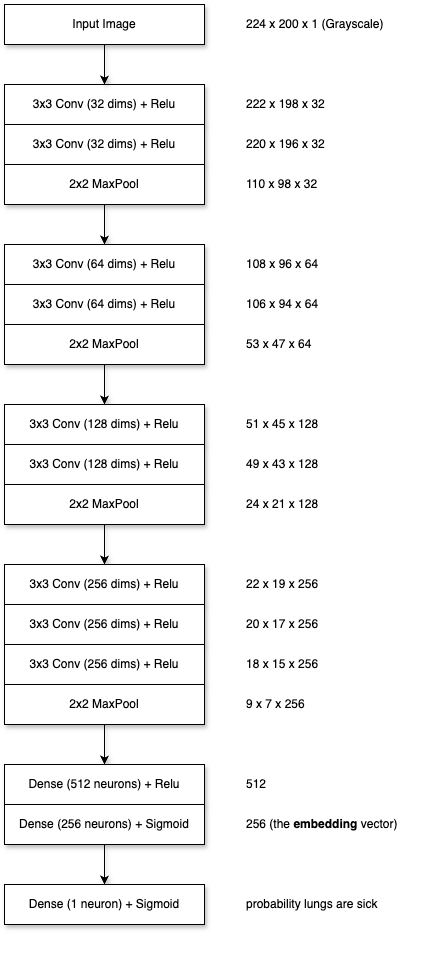
\includegraphics[width=0.45\linewidth, angle=90]{model_1.png}
  \caption{Binary Classification Model}
  \label{fig:model_1}
\end{figure}

\subsection{Experimental results}
We tweaked many aspects of our code during its journey to its final best form.

\textbf{Class imbalance:} the most challenging factor turned to be the class imbalance in the data.
When we matched the \textit{distribution of labels} in the train/val sets to 62.5\% (which is the distribution of labels in the test-set), the network achieved a final accuracy score of $\sim$96\% (measured on the test-set). Not altering the \textit{distribution of labels} in the train/val was (as expected) the worst - it limited the final accuracy to about $\sim$80\%. We decided (after e-mailing the course's TA) that "peeking" at the distribution of classes in the test-set was cheating, so we had two options: removing excess train/val data until the distribution was 50\%, or using different weights for each class in the loss function.
We tried both things, and achieved similar results, but the trimming of data into 50\% representation has yielded results a tad superior, giving us a final accuracy score of $\sim$92\% over the test-set.

\textbf{Optimizer:} we shortly plugged in other optimizer algorithms, and found they brought no improvement over Adam, or (like in the case of Adamax), resulted in inferior final test accuracy.

\textbf{Learning rate:} we tried other values other than 1e-4, and were surprised to find out they hurt the final network's test-accuracy to a significant degree. Even starting with 1e-4, and then lowering it on plateau to 1e-6, has led to immense over-fitting, causing the final accuracy score to drop to around 80\%.

\textbf{Weight transferring:} we tried copying the actual weights from the early layers of VGG16 (whose structure we adopted and tweaked), but it provided no help to the model final accuracy. We suspect it might happened due to our needs being specific to intricate blobs in the lungs, while VGG is more general form, and was designed to classify more general shapes; hence transferring its early weights would probably help detecting that the image \textit{is} lungs, but not further. Also, VGG was trained on RGB images, while our x-ray images are grayscale; using VGG might just lead to the model seeking information in the wrong places.

\textbf{Input image dimensions:} VGG uses 224x224 images. We measured the aspect ratio of our images to be roughly 1.124, which is better approximated in 224x200 images. However, after experimentation, it turned out that both resolution bring the network to the same final performance.

\textbf{Combating over-fitting:} over-fitting was a great source of tension in developing the model.
On one side, a bigger network is capable of more accurate results. On the other sides, given the limited size of the data (after balancing the classes, the train-set contained only 2,158 images to work with), a network too powerful would only memorize our data, achieving poor score on the test.
We applied many forms of train augmentations (shear, shift, rotation, brightness, zoom) and it did help.
We also stretched the size of the network (being its depth, the number of channels in each convolution layer, the number of neurons in the dense layers) to the absolute limit defined by the final test accuracy.

\textbf{"Hyper-Convergence":} it was difficult to draw rigorous scientific conclusions about the optimal network structure, as every experiment took half an our to run, and random luck carried an important ±5\% role in determining the network's final accuracy. Of course, repeating each experiment many times in parallel would allow us to reduce the variance, but our compute resources were limited.

In Figure~\ref{fig:model_1_history}, you can see the Loss fluctuating, dipping almost randomly at its lowest point on epoch 43. Indeed, different runs yielded different minimum points (meaning different final test accuracy). 

Our goal was maximizing test-accuracy, even at the cost of val-loss fluctuation in training, and even at the cost of having to run the notebook a few times and pick the best performing version. Overall, this way we were able to reach the highest test-accuracy of $\sim$92\% (again, this is without matching the labels distribution to the test. allowing it would make our model's score peak at $\sim$96\% test-accuracy).


\begin{figure}[H]
    \centering
    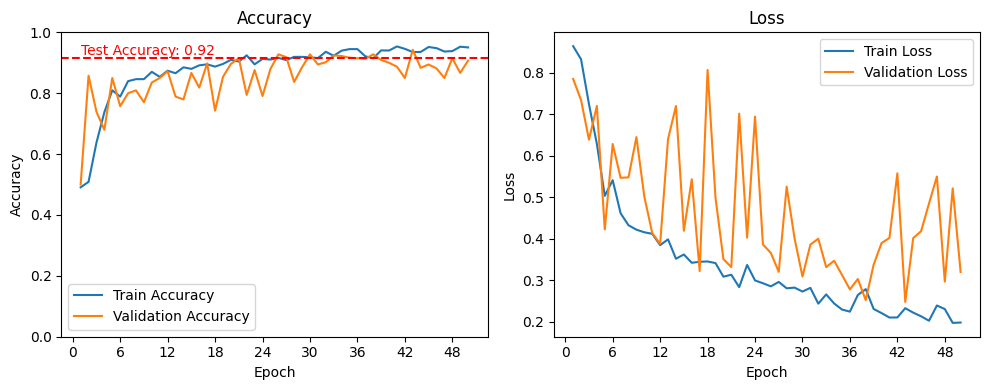
\includegraphics[width=1\linewidth]{model_1_history.png}
    \caption{Training the Binary Classification Model. Best Epoch is 43.}
    \label{fig:model_1_history}
\end{figure}

\subsection{Discussion}
To summarize the above points, we found that data is indeed key; a limited number of train examples posses an immense over-fitting barrier on the model size, which in turn sets a ceiling to the complexity of the patterns the model can learn. Matching the distribution of labels with the target test distribution also matters a lot; moving the final test accuracy between 80\% and 96\%. We found that exact image dimensions do not matter; we suspected that 224 could halve better (in max-pooling), and that 200 would better compliment the original aspect ratio; but in practice, every number in that range yields similar results. Predictability is hard; our models achieved different scores when we repeated the experiment on Kaggle. Please refer to the above sections for more thoughts, as this section cannot contain everything mentioned above.

\subsection{Code}

View the \href{https://www.kaggle.com/code/nitsanbh/lungs-x-ray}{notebook online}. There we're creating the binary classification model, training it, and assessing its performance. You'll also see answers to later questions on the same model, such as KNN in embedding-space, t-SNE, explainability, etc.

\
\section{Task 1.2: Multiclass Classification}

\subsection{Solution}
\subsubsection{General approach}
Describe your preferred approach to solve the problem. what alternatives you plan to try and why. 

\subsubsection{Design}
Provide some general information about your code, platform, how long it took you to train it, technical challenges you had, Loss functions, Optimizers, Architecture, and more.

\subsection{Experimental results}
Provide information about your experimental settings. What alternatives did you measure? Make sure this part is clear to understand, provide as much details as possible. Provide results with tables and figures.

\subsection{Discussion}
Provide some final words and summarize what you have found from running the experiments you described above. Provide some high level insights.

Note - your project will be evaluated for aspects, including the technique you selected, the rational of the experiments you decided to run, the insights you learned from this process and more. Remember, for the purpose of this course, the process that you demonstrate is very  important.

\subsection{Code}

Please provide a link to your colab notebook.


\
\section{Task 2: Model Embeddings and Visualization}

\subsection{Solution}
\subsubsection{General approach}
Describe your preferred approach to solve the problem. what alternatives you plan to try and why. 

\subsubsection{Design}
Provide some general information about your code, platform, how long it took you to train it, technical challenges you had, Loss functions, Optimizers, Architecture, and more.

\subsection{Experimental results}
Provide information about your experimental settings. What alternatives did you measure? Make sure this part is clear to understand, provide as much details as possible. Provide results with tables and figures.

\subsection{Discussion}
Provide some final words and summarize what you have found from running the experiments you described above. Provide some high level insights.

Note - your project will be evaluated for aspects, including the technique you selected, the rational of the experiments you decided to run, the insights you learned from this process and more. Remember, for the purpose of this course, the process that you demonstrate is very  important.

\subsection{Code}

Please provide a link to your colab notebook.


\
\section{Task 3: Anomaly Detection}

\subsection{Solution}

\subsubsection{The Problem}
\textit{In this task, you only have data for "healthy" images. Try to identify "sick" individuals using Anomaly Detection methods.}

This task is the most challenging. For once, the area the lungs occupy is only $\sim$20\% of each image's pixels, yet in it lies most (if not all) of the relevant data; The need to direct to model to focus on some moving $\sim$20\% area (the lungs) is clear. In addition, the size of the train-set this time was even more limited than in previous tasks, being only 1,079 "normal" images (after 20\% cut for validation).

\subsubsection{General approach}
We use an existing lungs-segmentation model to \textbf{concatenate a lungs-only image} next to each original image, and feed the resulting \textit{224 x 448} image as an input to our anomaly detection model. This helps our model focus on the lungs, while still seeing the "complete picture", which is more regular and predictable than just a blob of lungs floating in an all-black sea.

Our anomaly detection model is an \textbf{auto-encoder with a wide "bottle-neck"}. The "encoder" \uline{expends the dimensionality of the image, in an attempt to capture more patterns in it, rather than losing them in compression}.

The "encoder" (which more appropriately could be named "feature-expender") mostly consists of the early layers of VGG16 (with frozen weights); we only append one trainable convolution layer.

\begin{figure}[H]
  \centering
  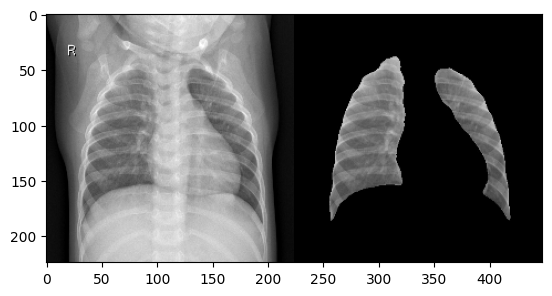
\includegraphics[width=0.8\linewidth]{concatenated-lungs-segmentation.png}
  \caption{Pre-processed Image for Anomaly Detection Model}
  \label{fig:concatenated-lungs-segmentation}
\end{figure}

\subsubsection{Design}

\textbf{Concatenating each Image alongside Lungs-Only Image:} after asking the TA for permission, we used a \href{https://www.kaggle.com/datasets/farhanhaikhan/unet-lung-segmentation-weights-for-chest-x-rays/data}{pre-trained lungs-segmentation U-Net}, to create a lungs-only version of each image in the dataset; we then concatenated the lungs-only version to the right of each original image.

\textbf{Wide Bottle-Neck "Auto-Encoder":} our "encoder" outputs tensors of shape \textit{112 x 224 x 32}; It's 8 times more dimensions than the input image, a mere \textit{224 x 448 x 1}. This makes our model "describe" an image with more details, rather than trying to compress it like a traditional auto-encoder.

\textbf{Custom Loss:} we compute SSIM on each half individually, then sum the results with weights. The reconstruction of lungs half is multiplied by \textit{0.75}, and the reconstruction of the original half is multiplied by \textit{0.25}.

\textbf{Augmentation:} apart from the lungs-segment concatenation, our pre-processing is minimal. It consists of slight variation in brightness and contrast, which we only apply to the original half.

\textbf{Anomaly Definition:} we compute the \textit{mean} ($\mu$) and \textit{standard deviation} ($\sigma$) of the validation loss. A test image is considered an anomaly if its reconstruction loss is NOT within $\mu\pm\sigma$.

\newpage
\subsection{Experimental results}

\textbf{Lungs-Segment Concatenation:} 
\begin{itemize}
\item When we trained the model on the \uline{original images alone}, it treated the entire x-ray (including the chin, armpits, spine, heart, and so on) the same; it resulted in \uline{negligible loss difference} between test-normal and test-sick.
\item When we trained the model on the \uline{lungs-segment images alone}, the pattern was too irregular; the model would always converge to the local minimum of constructing \uline{almost completely-black images}, no matter the loss we used (MSE, SSIM, cross-entropy, dice-loss).
\item Our solution was to \uline{concatenate} each original image alongside its lungs-segmented image, creating a dataset of 2:1 rectangular images. Our custom loss function \uline{makes the model focus on the lungs, while still using the "complete picture", which is easier to reproduce}.
\end{itemize}

\textbf{Loss Function:} 
\begin{quote}
Using the \uline{same loss strategy} (a weighted sum of the loss of each half), we tried \uline{replacing SSIM with MSE}. We were surprised to find it completely broke the model: instead of the regular result, where the standard deviation of the loss is an order of magnitude less than its mean, we got the opposite: a \uline{huge standard deviation, ten times the mean}. This nullified the possibility to distinguish between "normal" and "sick" based on reconstruction loss.
\end{quote}

\textbf{"Bottle-Neck" Shape:} 
\begin{quote}
In its final version, our model looks like a diamond, rather than a traditional auto-encoder's bow-tie. When we tried using an actual "bottle-neck" - being a vector of size 256 to 2048, the model's reconstructed images looked very blurred. Even in the best blurred version, the lungs were a monochromatic area; the model captured their contours, but missed 100\% of the details inside them.
\end{quote}

\textbf{Training Duration and Fine Tuning:}
\begin{quote}
When we transferred the first layers of VGG16, we froze its weights. We then let the model [TODO]
\end{quote}


\textbf{Measuring Improvement During Training:}
\begin{quote}
We relied on validation [TODO]
\end{quote}

\begin{figure}[H]
  \centering
  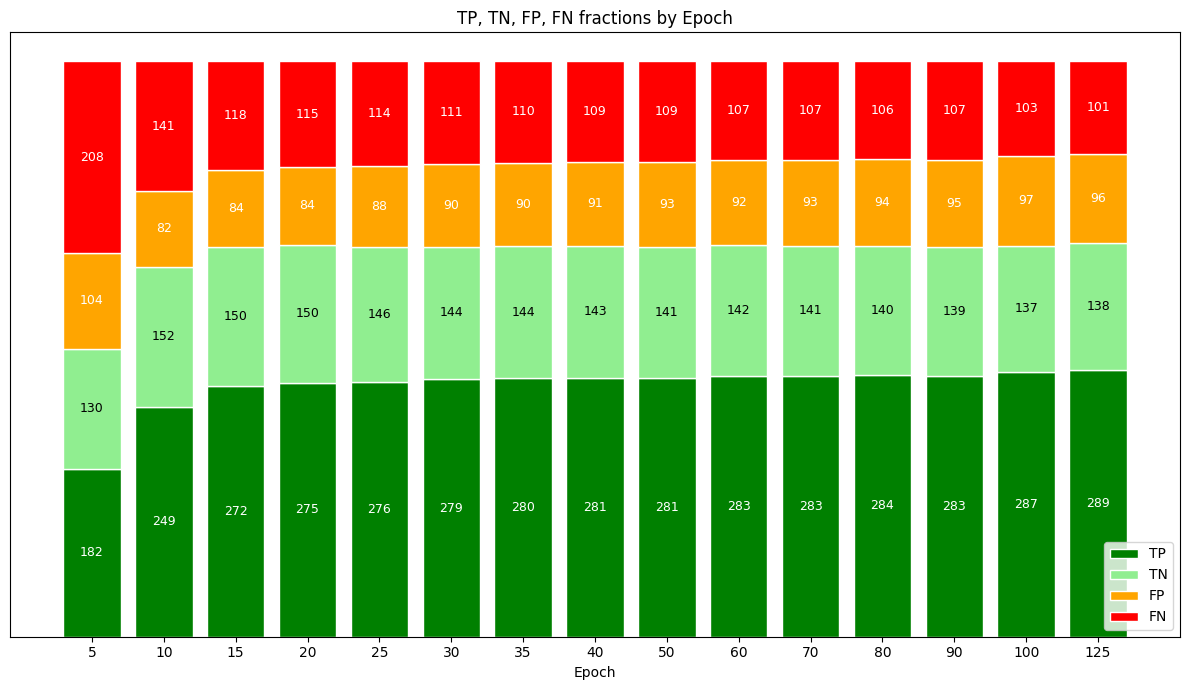
\includegraphics[width=1\linewidth]{confusion_by_epoch.png}
\end{figure}

\begin{figure}[H]
  \centering
  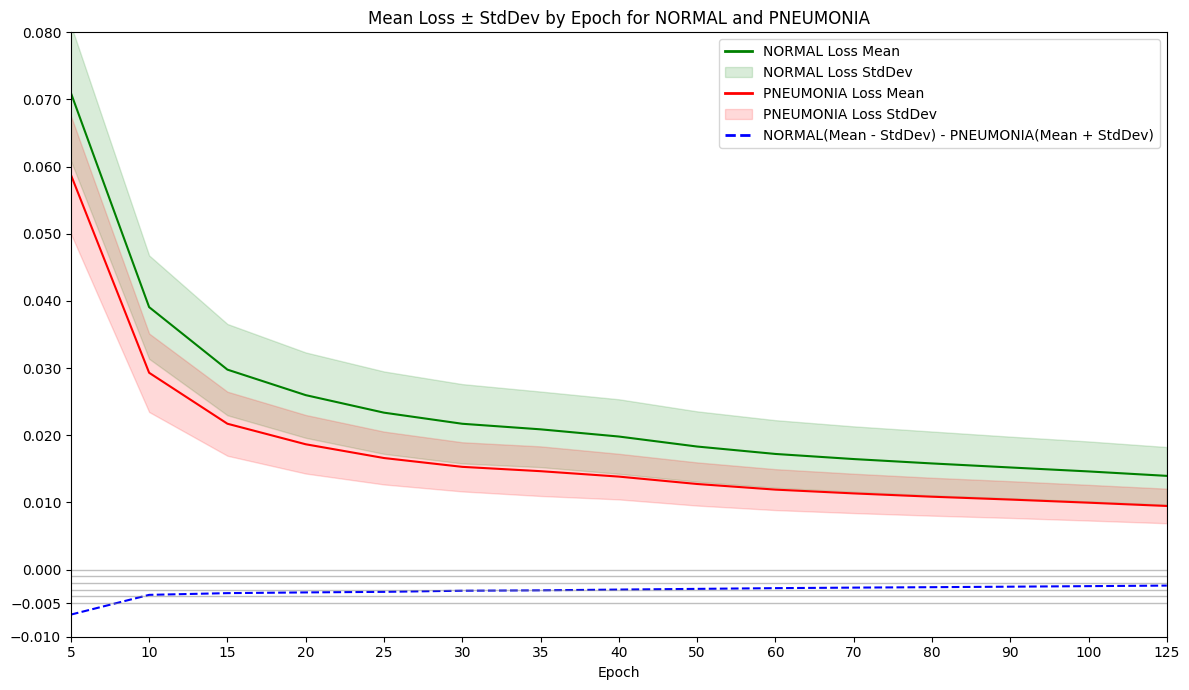
\includegraphics[width=1\linewidth]{losses_mean_std_by_epoch.png}
\end{figure}

\begin{figure}[H]
  \centering
  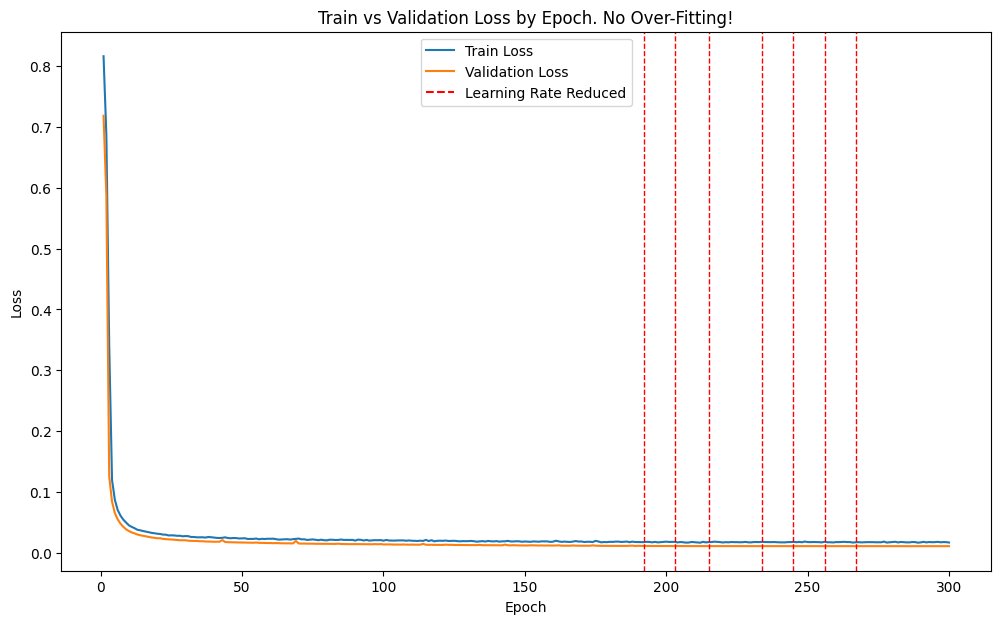
\includegraphics[width=1\linewidth]{train_val_loss_by_epoch.png}
\end{figure}

\begin{figure}[H]
  \centering
  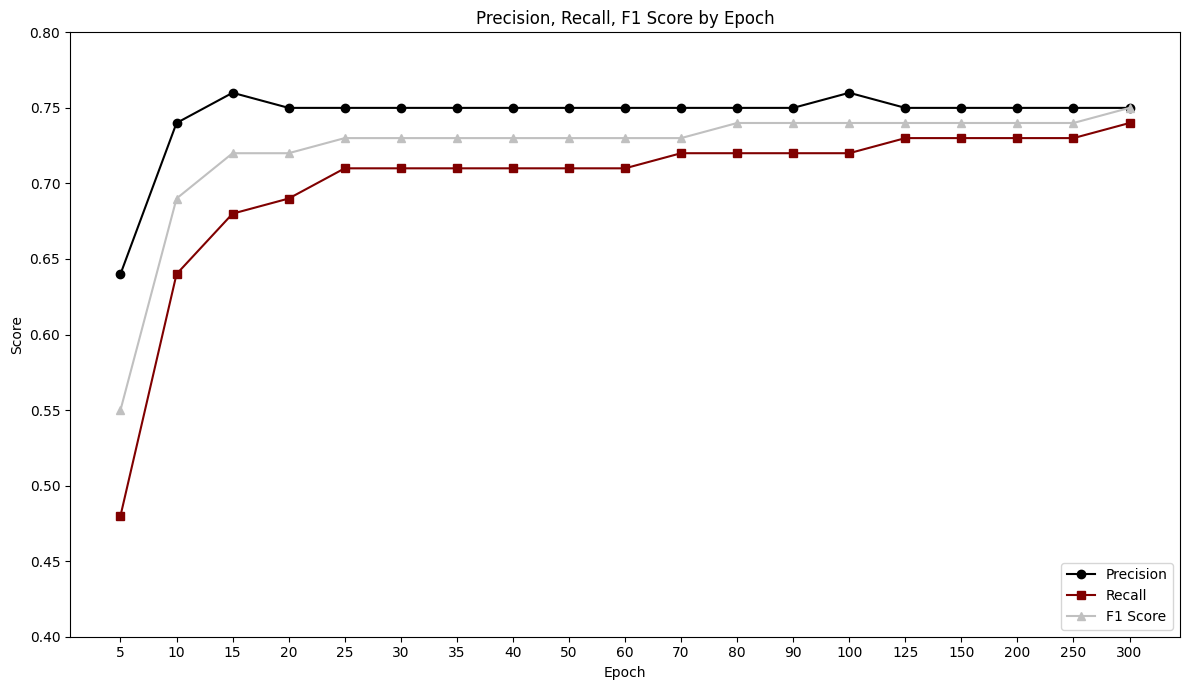
\includegraphics[width=1\linewidth]{scores_by_epoch.png}
\end{figure}

\subsection{Discussion}
Provide some final words and summarize what you have found from running the experiments you described above. Provide some high level insights.

Note - your project will be evaluated for aspects, including the technique you selected, the rational of the experiments you decided to run, the insights you learned from this process and more. Remember, for the purpose of this course, the process that you demonstrate is very  important.

\subsection{Code}

Please provide a link to your colab notebook.


\
\section{Task 4: Explainability in Deep Learning}

\subsection{Solution}
\subsubsection{General approach}
Describe your preferred approach to solve the problem. what alternatives you plan to try and why. 

\subsubsection{Design}
Provide some general information about your code, platform, how long it took you to train it, technical challenges you had, Loss functions, Optimizers, Architecture, and more.

\subsection{Experimental results}
Provide information about your experimental settings. What alternatives did you measure? Make sure this part is clear to understand, provide as much details as possible. Provide results with tables and figures.

\subsection{Discussion}
Provide some final words and summarize what you have found from running the experiments you described above. Provide some high level insights.

Note - your project will be evaluated for aspects, including the technique you selected, the rational of the experiments you decided to run, the insights you learned from this process and more. Remember, for the purpose of this course, the process that you demonstrate is very  important.

\subsection{Code}

Please provide a link to your colab notebook.

Good luck!!
\bibliographystyle{plain}
\bibliography{references}
\end{document}